\section{Actividad 4}

\subsection*{Considere la misma señal de mensaje y portadora del Ejercicio 2, pero utilice un modulador producto.} 

\subsection*{a) Expresar analíticamente $s(t)$ y $S(f)$. Graficar resultados y explicar cuál fue el cambio en la señal de salida del modulador.}
\bigskip

Se realiza la Modulación de Doble Banda Lateral con Portadora Suprimida(DSB-SC), está forma de modulación lineal es generada utilizando un modulador de producto, que simplemente multiplica la señal del mensaje $m(t)$ por la onda portadora $c(t)$.
\bigskip
\bigskip

La señal de mensaje y portadora del ejercicio 2 son las siguientes:
\bigskip

$m(t)=A_m\cos(2\pi f_m t)$ con $A_m=3$ V y $f_m=600$ Hz. 

$c(t)=A_c\cos(2\pi f_c t)$ con $A_c=10$ V y $f_c=1$ kHz.
\bigskip

La señal modulador producto es:
\bigskip

$s(t)=c(t) m(t)=A_c A_m\cos(2\pi f_m t) \cos(2\pi f_c t)$ 
\bigskip

Aplicando la propiedad trigonométrica del producto de cosenos, la expresión resultante es:
\bigskip

$s(t)=\frac{A_c A_m}{2}[\cos(2\pi (f_c-f_m t)+cos(2\pi (f_c+f_m t))]$ 
\bigskip

Mediante la transformada de fourier se obtiene $s(t)$ en el dominio de la frecuencia:
\[
S(f)=\tfrac{A_c A_m}{4}\big[\delta(f-(f_c+f_m))+\delta(f+(f_c+f_m))  \;+\; \delta(f-(f_c-f_m))+\delta(f+(f_c-f_m))\big]
\]

Reemplazando por valores numéricos:

\[
S(f)=\tfrac{30}{4}\big[\delta(f-1600+\delta(f+1600)  \;+\; \delta(f-400)+\delta(f+400)\big]
\]

En la Fig.\ref{fig:actividad_4a}  se observa las gráfica de s(t) tanto en el dominio del tiempo como en el dominio de la frecuencia.


\begin{figure}[H]
        \centering
        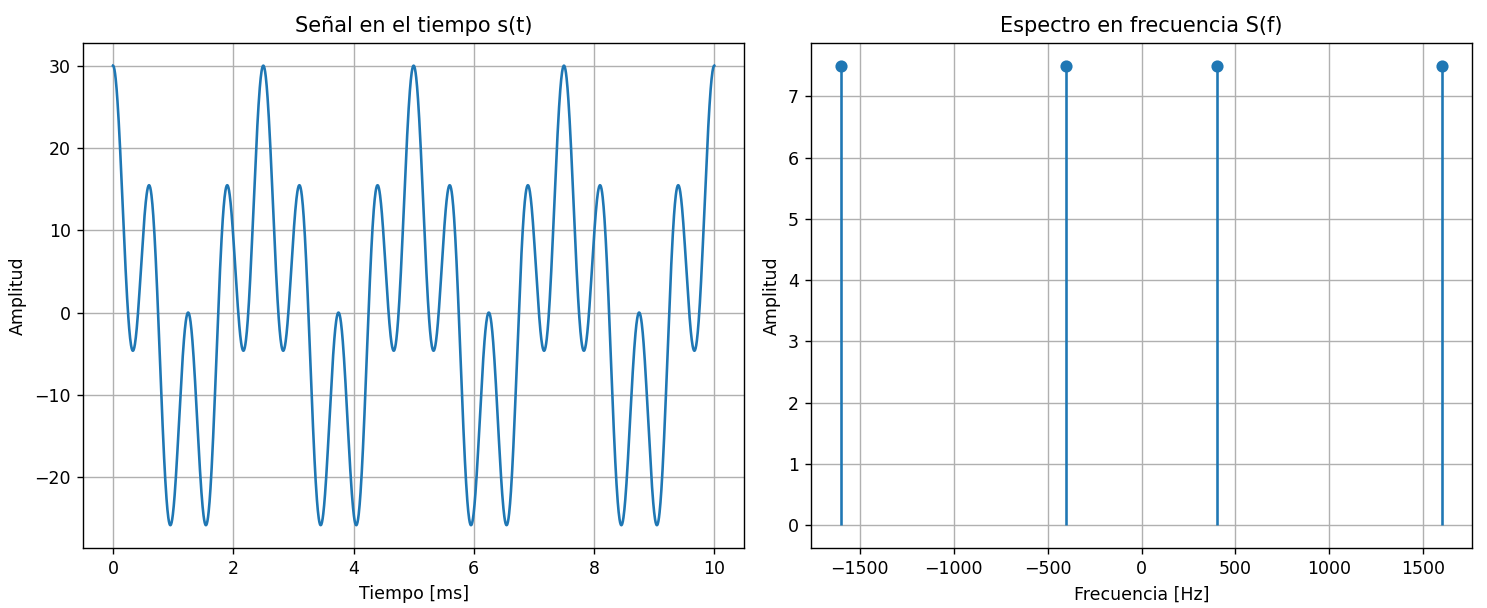
\includegraphics[width=0.9\textwidth]{imagenes/Parte_1/Actividad_4/actividad_4a.png}
        \caption{Gráfica de s(t) y S(f).}
        \label{fig:actividad_4a}
    \end{figure}



\subsection*{b) Considerando que la señal de salida del modulador se aplica a un detector coherente (ver Fig. \ref{fig:2}), y que las portadoras tanto en el transmisor como en el receptor se encuentran en perfecto sincronismo: obtener v(t) y graficar su espectro.}
\bigskip
Para obtener la señal $v(t)$ y su gráfico del espectro se realiza lo siguiente:

\[
v(t) = s(t)  A'_c \cos(2\pi f_c t+ \phi) =\frac{A_c A_m A'_c}{2}[\cos(2\pi (f_c-f_m t)+cos(2\pi (f_c+f_m t))] \cos(2\pi f_c t)
\]
\[
 =\frac{A_c A_m A'_c}{2}[\cos(2\pi (f_c-f_m t)\cos(2\pi f_c t)+cos(2\pi (f_c+f_m t))\cos(2\pi f_c t)] 
\]

Al estar en perfecto sincronismo $\phi=0$, ya que están en fase.
\bigskip

Al aplicar propiedad de producto de cosenos:

\[
v(t) = \frac{A_c A_m A'_c}{4}
\Big[
\cos\big(2\pi(2f_c - f_m)t\big)
+ 
\cos\big(2\pi(2f_c + f_m)t\big)
+ 
2\cos\big(2\pi f_m t\big)
\Big]
\]

Reemplazando por valores numéricos:

\[
v(t) = \frac{30}{4}
\Big[
\cos\big(2\pi(1400)t\big)
+ 
\cos\big(2\pi(2600)t\big)
+ 
2\cos\big(2\pi 600 t\big)
\Big]
\]

Al aplicar la transformada de Fourier se obtiene la expresión en frecuencia de $v(t)$:
\[
V(f) =
\frac{15}{4}
\Big[
\delta(f - 1400) + \delta(f + 1400)
\Big]
+
\frac{15}{4}
\Big[
\delta(f - 2600) + \delta(f + 2600)
\Big]
+
\frac{15}{2}
\Big[
\delta(f - 600) + \delta(f + 600)
\Big]
\]

\begin{figure}[H]
        \centering
        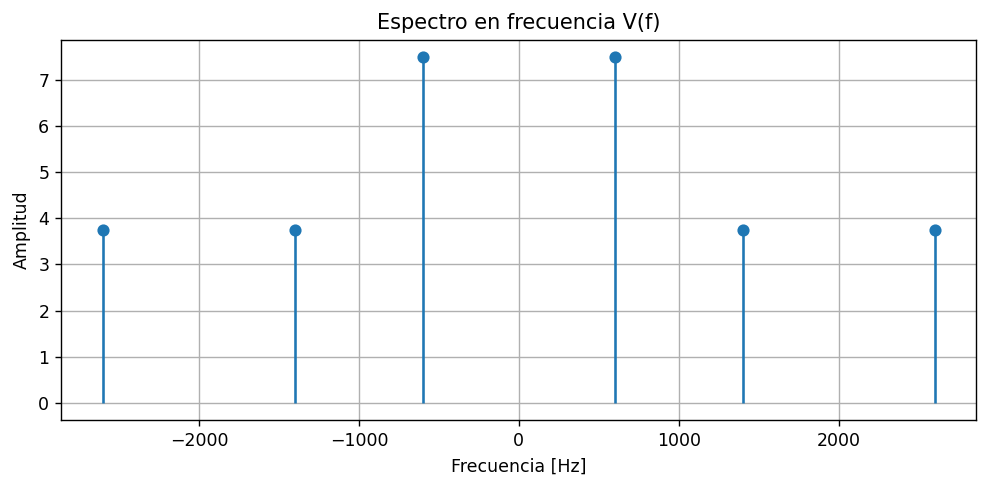
\includegraphics[width=0.9\textwidth]{imagenes/Parte_1/Actividad_4/actividad_4b.png}
        \caption{Gráfica de V(f).}
        \label{fig:2}
    \end{figure}

\bigskip
\subsection*{c) Ahora suponer que hay una diferencia de fase entre portadoras. Comentar por qué esto es importante y qué sucede en casos extremos.}
    
    \begin{figure}[H]
        \centering
        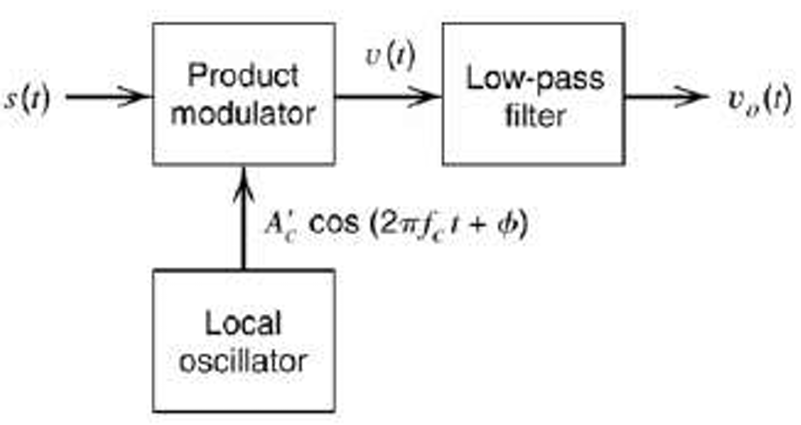
\includegraphics[width=0.4\textwidth]{imagenes/Parte_1/Actividad_2/fig2.png}
        \caption{Detector coherente.}
        \label{fig:2}
    \end{figure}
    